% Author: Natasha T. Petrus
% Document type: CV

\documentclass[letterpage]{article}

%%%%%%%%%%%%%%%%%%%%%%%%%%%%%%%%%%%%%
% DEFINE DEFAULT FONT STYLE
%%%%%%%%%%%%%%%%%%%%%%%%%%%%%%%%%%%%%
\usepackage{fontawesome}
\usepackage[defaultsans]{cantarell}
\usepackage[default,scale=0.95]{carlito}
\usepackage[T1]{fontenc}
\fontsize{10px}{0.45px}\selectfont
\usepackage{lmodern}

%%%%%%%%%%%%%%%%%%%%%%%%%%%%%%%%%%%%%
% DEFINE PAGE LAYOUT & SPACING
%%%%%%%%%%%%%%%%%%%%%%%%%%%%%%%%%%%%%
% For NO HYPHEN
\tolerance=1
\emergencystretch=\maxdimen
\hyphenpenalty=10000
\hbadness=10000
% NO HYPHEN END
\usepackage[top=0.55in, bottom=0.55in, left=0.55in,
right=0.85in]{geometry}
\usepackage{setspace} % for line spacing
\usepackage{vwcol} % unused - for columns with different widths
\usepackage{multicol} % unused - for columns with equal widths
% currently using minipage to create columns
\usepackage{enumitem} % for 'itemize' configuration
% http://ctan.org/pkg/enumitem
% bullet style for items in list:
\renewcommand\labelitemi{\rule[1mm]{0.33mm}{0.33mm}}  

%%%%%%%%%%%%%%%%%%%%%%%%%%%%%%%%%%%%%
% COLOR PACKAGE & PREDEFINED COLORS
%%%%%%%%%%%%%%%%%%%%%%%%%%%%%%%%%%%%%
\usepackage[dvipsnames]{xcolor}
\definecolor{white-smoke}{HTML}{F2F7F8}
\definecolor{arsenic}{HTML}{40424A}
\definecolor{light-sky-blue}{HTML}{87CBFF}
\pagecolor{white-smoke}
\AtBeginDocument{\color{arsenic}}

%%%%%%%%%%%%%%%%%%%%%%%%%%%%%%%%%%%%%
% OTHER PACKAGES
%%%%%%%%%%%%%%%%%%%%%%%%%%%%%%%%%%%%%
\usepackage{array,multirow,graphicx} % for tables
\usepackage{verbatim} % for multi-line comments
\usepackage{graphicx} % for rotating text boxes
\usepackage{tikz} % for drawing shapes & highlights
\usepackage{soul} % for text highlights/underlines
\setul{-0.5ex}{1ex} % set underline dimension
\setuloverlap{3pt} % how much line is sticking out
\setulcolor{light-sky-blue}
\usepackage{amssymb,amsmath}
\usepackage{mathabx} % for math symbols
\usepackage{ifxetex,ifluatex}
\usepackage{fixltx2e} % provides \textsubscript
\ifnum 0\ifxetex 1\fi\ifluatex 1\fi=0 % if pdftex
  \usepackage[T1]{fontenc}
  % Setup & declare Unicode characters
  \usepackage[utf8]{inputenc}
  \DeclareUnicodeCharacter{0160}{\^--}
\else % if luatex or xelatex
  \ifxetex
    \usepackage{mathspec}
  \else
    \usepackage{fontspec}
  \fi
  \defaultfontfeatures{Ligatures=TeX,Scale=MatchLowercase}
\fi
% use upquote if available, for straight quotes in verbatim
% environments
\IfFileExists{upquote.sty}{\usepackage{upquote}}{}
% use microtype if available
\IfFileExists{microtype.sty}{%
\usepackage{microtype}
\UseMicrotypeSet[protrusion]{basicmath}
% ^ disable protrusion for tt fonts
}{}
\usepackage[unicode=true]{hyperref}
\hypersetup{
            pdfborder={0 0 0},
            breaklinks=true}
\urlstyle{same}  % don't use monospace font for urls
\usepackage{graphicx,grffile} % for inserting pictures
\makeatletter
\def\maxwidth{\ifdim\Gin@nat@width>\linewidth\linewidth\else
\Gin@nat@width\fi}
\def\maxheight{\ifdim\Gin@nat@height>\textheight\textheight\else
\Gin@nat@height\fi}
\makeatother
% Scale images if necessary, so that they will not overflow 
% the page margins by default, and it is still possible to
% overwrite the defaults using explicit options in
% \includegraphics[width,height, ...]{}
\setkeys{Gin}{width=\maxwidth,height=\maxheight,keepaspectratio}
\IfFileExists{parskip.sty}{%
\usepackage{parskip}
}{% else
\setlength{\parindent}{0pt}
\setlength{\parskip}{6pt plus 2pt minus 1pt}
}
\setlength{\emergencystretch}{3em}  % prevent overfull lines
\providecommand{\tightlist}{%
  \setlength{\itemsep}{0pt}\setlength{\parskip}{0pt}}
\setcounter{secnumdepth}{0}
% Redefines (sub)paragraphs to behave more like sections
\ifx\paragraph\undefined\else
\let\oldparagraph\paragraph
\renewcommand{\paragraph}[1]{\oldparagraph{#1}\mbox{}}
\fi
\ifx\subparagraph\undefined\else
\let\oldsubparagraph\subparagraph
\renewcommand{\subparagraph}[1]{\oldsubparagraph{#1}\mbox{}}
\fi

\begin{document}
\thispagestyle{empty} % to remove page number
%%%%%%%%%%%%%%%%%%%%%%%%%%%%%%%%%%%%%
% HEADER: NAME & INFOMARTION
%%%%%%%%%%%%%%%%%%%%%%%%%%%%%%%%%%%%%
\begin{minipage}[c]{0.4\linewidth}
  \raggedright
  \textbf{\fontsize{37px}{1px}\selectfont\textsf{NATASHA}}\\
  \vspace{7px}
  {\fontsize{37px}{1px}\selectfont\textsf{PETRUS}}
\end{minipage}
\begin{minipage}{0.01\linewidth}
  % INTENTIONALLY LEFT BLANK
\end{minipage}
\:\:\:\:\: % space between minipages
\begin{minipage}[t]{0.31\linewidth}
  \raggedleft
  \vspace*{-30px}
  natashapetr.us\enspace\faGlobe\\
  hire@npetr.us\enspace\faPaperPlane\\
  linkedin.npetr.us\enspace\faLinkedin\\
  github.npetr.us\enspace\faGithubAlt
\end{minipage}
\:\:\:\:\: % space between minipages
\begin{minipage}[c]{0.2\linewidth}
  \raggedright
  \begin{tikzpicture}
    \fill[light-sky-blue] (0,2.2) circle (1.2);
    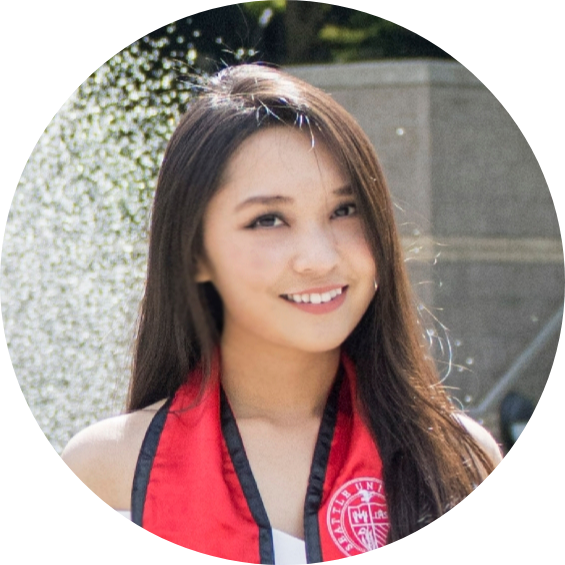
\includegraphics[width=1\linewidth]{assets/images/profile.png}
  \end{tikzpicture}
\end{minipage}
\vspace*{20px}\\ % space between header and content
%------------------------------------
% First Column
%------------------------------------
\begin{minipage}[t]{0.424\linewidth}
\vspace{0pt}
%%%%%%%%%%%%%%%%%%%%%%%%%%%%%%%%%%%%%
% EDUCATION HISTORY
%%%%%%%%%%%%%%%%%%%%%%%%%%%%%%%%%%%%%

\textbf{\fontsize{14px}{1px}\selectfont
  \ul{E D U C A T I O N}
}\\
\vspace{5px}\\
\textcolor{gray}{September 2015 - June 2017}\\
\textbf{\textsf{Seattle University - Seattle, WA}}\\
\textbf{Bachelor of Science in Electrical Engineering}\\
\textbf{Summa Cum Laude}\\
\textbf{GPA: 3.99 / 4.00}
\begin{itemize}[leftmargin=*,labelindent=5mm,labelsep=7mm]
\item
  Messina Merit Scholarship
\item
  IEEE-HKN Mu Iota Chapter
  {\begin{list}{}{}
    \item
    	Web Correspondent
  \end{list}}
\item
  Alpha Sigma Nu Jesuit Honor Society
  {\begin{list}{}{}
    \item
      Top 4\% of Senior Class
  \end{list}}
\item
  Tau Beta Pi Engineering Honor Society
\item
  Tau Sigma National Honor Society
\item
  President's and Dean's Lists
  {\begin{list}{}{}
    \item
    	September 2015 - June 2017
  \end{list}}
\end{itemize}
\vspace{7px}

%% College
\textcolor{gray}{September 2013 - June 2015}\\
\textbf{\textsf{North Seattle College - Seattle, WA}}\\
\textbf{Associate of Science Degree }

%\begin{itemize}[leftmargin=*,labelindent=5mm,labelsep=7mm] 
%\item
%  Phi Theta Kappa Honor Society
%  {\begin{list}{}{}
%    \item
%    	March 2014 - Present
%  \end{list}}
%\item
%  Vice President/Dean's List\\
%  September - December 2013
%\item
%  President's List\\
%  January 2014 - June 2015
%\end{itemize}
\vspace{19px}

%%%%%%%%%%%%%%%%%%%%%%%%%%%%%%%%%%%%%
% COMPETENCIES / TECHNICAL SKILLS
%%%%%%%%%%%%%%%%%%%%%%%%%%%%%%%%%%%%%
\textbf{\fontsize{14px}{1px}\selectfont
  \ul{C O M P E T E N C I E S}
}\\
\vspace{0px}\\
\begin{minipage}[t]{0.01\linewidth}
% INTENTIONALLY LEFT BLANK
\end{minipage}
\: % space between left margin and text

\begin{minipage}[]{0.9\linewidth}
\linespread{0.895}\selectfont

\setlength{\tabcolsep}{0pt} % no spacing between columns
\begin{tabular}{p{0.1\linewidth}p{0.05\linewidth}p{0.3\linewidth}p{0.45\linewidth}}
  \parbox[t]{2mm}{\multirow{3}{*}{\LARGE \rotatebox[origin=c]{90}{\textcolor{lightgray}{L\:\:A\:\:N\:\:G}}}}
  &
  &
  English &
  \begin{tikzpicture}
    \fill[light-sky-blue] (0,0) circle (0.125);
    \fill[light-sky-blue] (0.6,0) circle (0.125);
    \fill[light-sky-blue] (1.2,0) circle (0.125);
    \fill[light-sky-blue] (1.8,0) circle (0.125);
    \fill[light-sky-blue] (2.4,0) circle (0.125);
  \end{tikzpicture} \vspace*{5px} \\ && 
  Indonesian &
  \begin{tikzpicture}
    \fill[light-sky-blue] (0,0) circle (0.125);
    \fill[light-sky-blue] (0.6,0) circle (0.125);
    \fill[light-sky-blue] (1.2,0) circle (0.125);
    \fill[light-sky-blue] (1.8,0) circle (0.125);
    \fill[light-sky-blue] (2.4,0) circle (0.125);
  \end{tikzpicture} \vspace*{5px} \\ && 
  French &
  \begin{tikzpicture}
    \fill[light-sky-blue] (0,0) circle (0.125);
    \fill[light-sky-blue] (0.6,0) circle (0.125);
    \fill[lightgray] (1.2,0) circle (0.125);
    \fill[lightgray] (1.8,0) circle (0.125);
    \fill[lightgray] (2.4,0) circle (0.125);
  \end{tikzpicture} \vspace*{5px} \\ && 
  Chinese &
  \begin{tikzpicture}
    \fill[light-sky-blue] (0,0) circle (0.125);
    \fill[lightgray] (0.6,0) circle (0.125);
    \fill[lightgray] (1.2,0) circle (0.125);
    \fill[lightgray] (1.8,0) circle (0.125);
    \fill[lightgray] (2.4,0) circle (0.125);
  \end{tikzpicture} \vspace*{10px} \\ && 
  \multicolumn{2}{p{0.75\linewidth}}{
    \raggedright
    C\#,
    HTML +  CSS,
    JavaScript (jQuery, Typescript, ReactJS, React Native, Knockout, AngularJS),
    SQL,
    LaTeX,
    MATLAB,
    C,
    C++,
    Python,
    Java + Scala,
    PHP,
    VHDL,
    MIPS Assembly Language
  }
\end{tabular}
\vspace*{14px}\\
% change textbullet style
\renewcommand{\textbullet}{\rule[1mm]{0.33mm}{0.33mm}}
% add ability to use P instead of p for text alignment (left)
\newcolumntype{P}[1]{>{\raggedright\arraybackslash}p{#1}}
\begin{tabular}{p{0.1\linewidth}p{0.05\linewidth}p{0.1\linewidth}P{0.65\linewidth}}
  \parbox[t]{2mm}{\multirow{3}{*}{\LARGE \rotatebox[origin=c]{90}{\textcolor{lightgray}{S\:\:K\:\:I\:\:L\:\:L}}}}
  &
  &
  \textbullet &
  Full-stack web \& mobile apps design and development
  \\ &&  \textbullet &
  PCB design and soldering
  \\ &&  \textbullet &
  Custom IC layout design
  \\ &&  \textbullet &
  FPGA programming and testing
  \\ &&  \textbullet &
  Strong organizational, analytical, interpersonal,
      presentation, \& technical writing skills
  \\ &&  \textbullet &
  Experienced in graphic design
\end{tabular}
\vspace*{14px}\\
\begin{tabular}{p{0.1\linewidth}p{0.05\linewidth}p{0.75\linewidth}}
  \parbox[t]{2mm}{\multirow{3}{*}{\LARGE \rotatebox[origin=c]{90}{\textcolor{lightgray}{T\:\:E\:\:C\:\:H}}}}
  &
  &
  \raggedright
  Visual Studio,
  Visual Studio Code,
  IntelliJ IDEA,
  Git/GitHub/GitLab,
  SQL/RDBMS (MySQL, PostgreSQL),
  NoSQL (MongoDB, Redis),
  Jenkins,
  RabbitMQ,
  Docker,
  AWS (OpsWorks, Elasticsearch, ElastiCache)
  CircleCI,
  Expo,
  MS Office,
  NI Multisim,
  NI Ultiboard,
  AutoCAD, 
  Solidworks
\end{tabular}
\end{minipage}

\end{minipage}
%------------------------------------
% Second Column
%------------------------------------
\begin{minipage}[t]{0.63\linewidth}
\vspace{0pt}
%%%%%%%%%%%%%%%%%%%%%%%%%%%%%%%%%%%%%
% RELEVANT EXPERIENCE
%%%%%%%%%%%%%%%%%%%%%%%%%%%%%%%%%%%%%
\textbf{\fontsize{14px}{1px}\selectfont
  \ul{R E L E V A N T \:\: E X P E R I E N C E}
}\\

%% Kit.com: Software Engineer
\vspace{7px}
\textcolor{gray}{September 2019 - Present}\\
\textbf{\textsf{Software Engineer for Kit.com}}\\
\raggedright
Currently responsible for infrastructure migration,
maintaining existing functionality, as well as implementing
new features following Geniuslink's acquisition of Kit.com.

%% Geniuslink: Software Engineer
\vspace{7px}
\textcolor{gray}{October 2017 - Present}\\
\textbf{\textsf{Software Engineer at Geniuslink}}
\begin{itemize}[leftmargin=*,labelindent=1mm,labelsep=0mm]
\item
  \begin{quote}
  \raggedright
  Has increased the number of automated integration tests
  against the company's web applications by more than 3000\% thus far
  \end{quote}
\item
  \begin{quote}
  \raggedright
  Allowed all integration tests to be run against any
  environment easily through Jenkins and greatly
  assisted in making Canary testing possible
  \end{quote}
\item
  \begin{quote}
  \raggedright
  Designed and developed Geniuslink's REST API v3
  \end{quote}
\item
  \begin{quote}
  \raggedright
  Designed and programmed the preliminary version of the company's mobile
  application using React Native
  \end{quote}
\item
  \begin{quote}
  \raggedright
  Frontend/backend work using C\#, Typescript/JS,
  jQuery, and Knockout
  \end{quote}
\end{itemize}

%% HCI Technologies/Microsoft: Game Tester
\vspace{7px}
\textcolor{gray}{September - October 2017}\\
\textbf{\textsf{Game Tester at HCL Technologies/Microsoft}}\\
\raggedright
Worked within HCL Technologies' CERT lab, partnering with
Microsoft, to certify pre-released Xbox games were
up to specified software and platform standards.

%% Senior Design / Interdisciplinary Project: T-Mobile
\vspace{7px}
\textcolor{gray}{September 2016 - June 2017}
\textcolor{light-sky-blue}{\quad {\small [ patent pending ]}}
\\
\textbf{\textsf{Interdisciplinary Project:
		T-Mobile Compact Robotic System}}\\
\raggedright
Refined handset validation testing for T-Mobile via robotic
implementation;\\reduced manufacturing cost by at least 50\%,
reduced physical size by at least 60\%, and improved
power efficiency.\\
\begin{itemize}[leftmargin=*,labelindent=1mm,labelsep=0mm]
\item
  \begin{quote}
  \raggedright
  Designed and manufactured two working prototypes within
  a year using SolidWorks (3D modeling)
  \end{quote}
\item
  \begin{quote}
  \raggedright
  Programmed in C++,
  used OpenCV and LabView for image processing
  \end{quote}
\end{itemize}

%% VLSI Project: 4-bit ALU
\vspace{7px}
\textcolor{gray}{March - June 2017}\\
\textbf{\textsf{VLSI Project: ALU Integrated Circuit Design}}\\
\raggedright
Designed the 3D layout of an ALU chip from transistor level
using Electric VLSI.

%% Independent Study Project
\vspace{7px}
\textcolor{gray}{January - March 2017}\\
\textbf{\textsf{Independent Study: 13.56MHz RFID on Ettus N210 SDR}}\\
\raggedright
Implemented the ISO 18000 13.56 MHz RFID standard on software defined
radios with LFRX and LFTX daughterboards.

%% Aneka Elektrindo Panel
\vspace{7px}
\textcolor{gray}{July - August 2016}\\
\textbf{\textsf{Electrical Engineering Intern
at PT Aneka Elektrindo Panel}}\\
\raggedright
Designed and built circuit panels based on client's
specifications using AutoCAD.

%% Global Visionaries
\vspace{7px}
\textcolor{gray}{October 2015 - June 2016}\\
\textbf{\textsf{Internship: IT Manager at Global Visionaries}}\\
\begin{itemize}[leftmargin=*,labelindent=1mm,labelsep=0mm]
\item
  \begin{quote}
  \raggedright
  Set up an online auction and created a donation page to
  support the educational needs of underprivileged youth
  \end{quote}
\item
  \begin{quote}
  \raggedright
  Provided network security strategies and conducted staff
  training
  \end{quote}
\end{itemize}

%% MATLAB Tutor & Grader
\vspace{7px}
\textcolor{gray}{January - March 2016}\\
\textbf{\textsf{MATLAB Teaching Assistant at Seattle University}}
\begin{itemize}[leftmargin=*,labelindent=1mm,labelsep=0mm]
\item
  \begin{quote}
  \raggedright
  Provided in-class help and out-of-class tutoring sessions
  \end{quote}
\item
  \begin{quote}
  \raggedright
  Graded weekly projects and assignments
  \end{quote}
\end{itemize}

\end{minipage}

\end{document}